\documentclass[9pt,landscape]{memoir}
\usepackage{multicol}
\usepackage{calc}
\usepackage{ifthen}
\usepackage[landscape]{geometry}
\usepackage{hyperref,siunitx}
\usepackage{amssymb,amsmath,verbatim,graphicx,enumitem,microtype,upquote,units,booktabs,siunitx,hyperref}

% To make this come out properly in landscape mode, do one of the following
% 1.
%  pdflatex latexsheet.tex
%
% 2.
%  latex latexsheet.tex
%  dvips -P pdf  -t landscape latexsheet.dvi
%  ps2pdf latexsheet.ps


% If you're reading this, be prepared for confusion.  Making this was
% a learning experience for me, and it shows.  Much of the placement
% was hacked in; if you make it better, let me know...


% 2008-04
% Changed page margin code to use the geometry package. Also added code for
% conditional page margins, depending on paper size. Thanks to Uwe Ziegenhagen
% for the suggestions.

% 2006-08
% Made changes based on suggestions from Gene Cooperman. <gene at ccs.neu.edu>


% To Do:
% \listoffigures \listoftables
% \setcounter{secnumdepth}{0}


% This sets page margins to .5 inch if using letter paper, and to 1cm
% if using A4 paper. (This probably isn't strictly necessary.)
% If using another size paper, use default 1cm margins.
\ifthenelse{\lengthtest { \paperwidth = 11in}}
	{ \geometry{top=.5in,left=.5in,right=.5in,bottom=.5in} }
	{\ifthenelse{ \lengthtest{ \paperwidth = 297mm}}
		{\geometry{top=1cm,left=1cm,right=1cm,bottom=1cm} }
		{\geometry{top=1cm,left=1cm,right=1cm,bottom=1cm} }
	}

% Turn off header and footer
\pagestyle{empty}
\renewcommand{\familydefault}{\sfdefault}
\setlist[itemize]{leftmargin=0pt, noitemsep, before={\vspace*{-.25\baselineskip}}, after={\vspace*{-\baselineskip}}}
\setlist[enumerate]{leftmargin=0pt, noitemsep, before={\vspace*{-.25\baselineskip}}, after={\vspace*{-\baselineskip}}}

% Redefine section commands to use less space
\makeatletter
\renewcommand{\section}{\@startsection{section}{1}{0mm}%
                                {-1ex plus -.5ex minus -.2ex}%
                                {0.5ex plus .2ex}%x
                                {\normalfont\large\bfseries}}
\renewcommand{\subsection}{\@startsection{subsection}{2}{0mm}%
                                {-1explus -.5ex minus -.2ex}%
                                {0.5ex plus .2ex}%
                                {\normalfont\normalsize\bfseries}}
\renewcommand{\subsubsection}{\@startsection{subsubsection}{3}{0mm}%
                                {-1ex plus -.5ex minus -.2ex}%
                                {1ex plus .2ex}%
                                {\normalfont\small\bfseries}}
\makeatother

% Define BibTeX command
\def\BibTeX{{\rm B\kern-.05em{\sc i\kern-.025em b}\kern-.08em
    T\kern-.1667em\lower.7ex\hbox{E}\kern-.125emX}}

% Don't print section numbers
\setcounter{secnumdepth}{0}


\setlength{\parindent}{0pt}
\setlength{\parskip}{0pt plus 0.5ex}


% -----------------------------------------------------------------------

\begin{document}

\raggedright
\footnotesize
\begin{multicols}{3}


% multicol parameters
% These lengths are set only within the two main columns
%\setlength{\columnseprule}{0.25pt}
\setlength{\premulticols}{1pt}
\setlength{\postmulticols}{1pt}
\setlength{\multicolsep}{1pt}
\setlength{\columnsep}{2pt}

\begin{center}
     \Large{\textbf{Statistics Crib Sheet}} \\
\end{center}

\section{Introduction}
\begin{equation*}
    \bar{X} = \frac{1}{n} \sum _{i = 1} ^{n} x_i
\end{equation*}

\begin{align*}
    s^2 &= \frac{1}{n - 1} \sum _{i = 1} ^n \left( x_1 - \bar{X} \right)^2 \\
        &= \frac{1}{n - 1} \sum _{i = 1} ^n \left( x_1^2 - n\bar{X}^2 \right) \\
    s   &= \sqrt{s^2} \\
        &= \sqrt{\frac{1}{n - 1} \sum _{i = 1} ^n \left( x_1^2 - n\bar{X}^2 \right)} \\
        &= \sqrt{\frac{1}{n - 1} \sum _{i = 1} ^n \left( x_1^2 - n\bar{X}^2 \right)}
\end{align*}

\begin{align*}
    \bar{Y} &= a + b\bar{X} \\
    S^2_Y   &= b^2 s_X^2 \\
    S_Y     &= |b|s_x
\end{align*}

\begin{equation*}
    \text{$p$th percentile} = \frac{p}{100}\left( n +1 \right)
\end{equation*}

\begin{itemize}
    \item A histogram is perfectly symmetric if its right half is a mirror image of its left half.
    \item A histogram with a long right-hand tail is called skewed to the right or positively skewed.
    \item A histogram with a long left-hand tail is called skewed to the left or negatively skewed.
    \item A histogram is unimodal if it has only one peak, or mode. A histogram is bimodal if it has two peaks, or mode. A bimodal histogram, in some cases, indicates that the sample can be divides into two subsamples that differ from each to other. If there are more than two peaks in a histogram, then it is said to be multimodal.

    \item Steps in construction of a boxplot
    \begin{enumerate}
        \item Computer the median and first and third quartiles of the sample. Indicate these with horizontal lines.
        \item Find largest sample value that no more than $1.5 IQR$ above the third and quartile, and smallest value less than the first quartile.
        \item Plot points. (first quartile) $1.5 IQR < x < 1.5 IQR$ (third quartile)
    \end{enumerate}
\end{itemize}

\begin{center}
    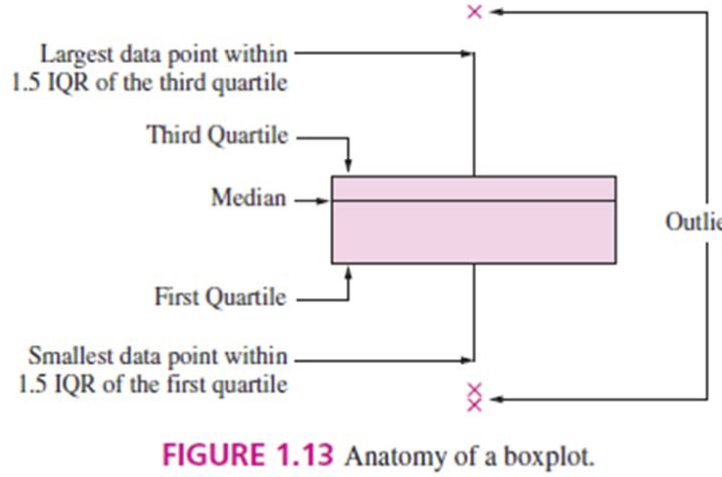
\includegraphics[width=.5\columnwidth]{boxplot.jpg}
\end{center}

\section{Probability}
\begin{enumerate}
    \item Let $S$ be a sample space. Then $P(S) = 1$
    \item For any event, $0 \leq P(A) \leq 1$
    \item If $A$ and $B$ are mutually exclusive events, then $P(A \cup B) = P(A) + P(B)$.
\end{enumerate}

\subsection{Complement Rule}
\begin{description}
    \item[Complement Rule] $P(A^C) = 1 - P(A)$
    \item[Addition Rule] $P(A \text{ or } B) = P(A \cup B) = P(A) + P(B) - P(A \cap B)$
\end{description}

\begin{itemize}
    \item The probability with equally likely outcomes has a probability $P(A) = \frac{K}{N}$
    \item The number of permutation of k objects chosen from a group of $n$ objects is

        \begin{equation*}
            P_{n,k} = \frac{n!}{(n - k)!}
        \end{equation*}

    \item The number of combinations of $k$ objects chosen from a group of $n$ objects

        \begin{equation*}
            {n \choose k} = \frac{n!}{k!(n - k)!}
        \end{equation*}

    \item The number of ways of dividing a group of $n$ objects into groups of $k_1$, $k_2$, $\ldots$, $k_n$

        \begin{equation*}
            \frac{n!}{k_1! k_2! \ldots k_r!}
        \end{equation*}

    \item A probability that is based on a part of a sample space called a conditional probability.

        \begin{equation*}
            P(A|B) = \frac{P(A \cup B)}{P(B)}
        \end{equation*}

    \item If $A$ and $B$ are two events with $P(B) \neq 0$, then

        \begin{align*}
            P(A \cup B) &= P(B)P(A|B) \quad \forall B \in\mathbb{R}, B \neq 0\\
                        &= P(A)P(B|A) \quad \forall A \in\mathbb{R}, A \neq 0
        \end{align*}

    \item Let $A$ and $B$ be events with $P(A) \neq 0$, $P(A^C) \neq 0$, and $P(B) \neq 0$.

        \begin{equation*}
            P(A|B) = \frac{P(B|A)P(A)}{P(B|A)P(A) + P(B|A^C)P(A^C)}
        \end{equation*}

    Generally,

            \begin{equation*}
                P(A_k|B) = \frac{P(B|A_k)P(A_k)}{\sum_{i = 1} ^n P(B|A_i)P(A_i)}
            \end{equation*}

        \item The cumulative distribution function of r.v $X$ is defined as:

            \begin{equation*}
                F(X) = P(X \leq x) = \sum P(X \leq t) = \sum P(t)
            \end{equation*}

        \item Let $X$ be a discrete random variable with probability mass function $p(x) = P(X \leq x$/ The \textbf{Mean} is given by

            \begin{align*}
                \mu_x &= \sum xP(X = x) \\
                      &= \int _{-\infty} ^{\infty} x\,f(x)\,dx
            \end{align*}

        \item The \textbf{variance} of $X$ is given by

            \begin{align*}
                \sigma^2 _X &= \sum (x - \mu_x)^2 P(X = x) = \sum x^2 P(X = x) - \mu_x^2 \\
                            &= \int _{-\infty} ^{\infty} (x - \mu_x)^2 f(x)\,dx = \int _{-\infty} ^{\infty} x^2\,f(x)\,dx - \mu_x^2
            \end{align*}

        \item The median of $X$ is the point $x_m$ that solves the equation

            \begin{equation*}
                F(x_m) = P(X \leq x_m) = \int _{-\infty} ^{x_m} f(x)\, dx = 0.5
            \end{equation*}

        \item The $p$th percentile is

            \begin{equation*}
                F(x_m) = P(X \leq x_m) = \int _{-\infty} ^{x_m} f(x)\, dx = \frac{p}{100}
            \end{equation*}
        \item If a random variable $X$ is multiplied by a constant $a$ and then added to another constant $b$, then we have a new random variable $Y$, where

            \begin{align*}
                Y &= a*X + b \\
                E(Y) &= \mu_y = a * E(X) + b \\
                Var(Y) &= \sigma_y^2 = a^2 * var(X) \\
                \sigma_Y &= |a|\sigma_x
            \end{align*}

        \item If $X_1, \ldots, X_n$ is a simple random sample from a population with mean $\mu$ and variance $\sigma^2$, then the sample mean $\bar{X}$ is a random variable with

            \begin{align*}
                \mu_{\bar{X}} &= \mu \\
                \sigma_{\bar{X}}^2 &= \frac{\sigma^2}{n}
            \end{align*}

        The standard deviation of $\bar{X}$ is

            \begin{equation*}
                \sigma_{\bar{X}} = \frac{\sigma}{\sqrt{n}}
            \end{equation*}
\end{itemize}


% \section{Definitions}
\begin{description}
    % \item[Population] A population is the entire collection of objects or outcomes about which information is sought. Denote the number of elements in the population is by $N$.
    % \item[Sample] A sample is a subset of population, containing the objects or outcomes that are actually observed. Typically denote sample size by $n$.
    % \item[Observation] is the observed value of a particular variable at a particular period. Observations concern a set of individuals from a population.
    % \item[Data Set] A data set is a collection of observations.
    % \item[Individuals] The individuals are the objects described by a set of data.
    % % \item[Information] Information is organized as a set of variables.
    % % \item[Variable] A variable is a characteristic of an individual whose value may differ between individuals
    % \item[Simple Random Sample (SRS)] A simple random sample of size $n$ is a sample chosen by a method in which each collection of the $n$ population items is equally likely to make up the sample.
    % \item[Sample of Convenience] is a sample that is obtained in some convenient way, and not drawn by a well-defined random method.
    % \item[Tangible Population] the population consisted of actual physical objects. (customers, lottery)
    % \item[Conceptual population] A simple random sample may consist of values obtained from a process under identical experimental conditions. In this case, the sample comes from a population that consists of all the values that might possibly have been observed. Such a population is called a conceptual population. (weights of a rock on a sensitive scale)
    % \item[Weighted sampling] Some items are given a greater chance of being selected than others.
    % \item[Stratified random sample] The population is divided up into subpopulations, called \textit{strata}, and simple random sample is drown from each stratum
    % \item[Quantitative (numerical) data] is data that can be measured.
    % \item[Qualitative (categorical) data] is data that can be observed but not measured or quantified.
    % \item[Controlled experiments] Experiments are designed to determine the effect of changing one or more factors on the value of the response.
    % \item[Observational studies] The experimenter simply observes the levels of the factor as they are, without having any control over them.
    % \item[Sample proportion (relative frequencies)] The sample proportion is the frequency divided by the sample size $\text{relative frequencies} = \frac{\text{frequency}}{\text{sample size}}$
    % \item[Experiment] An experiment is a process that results in an outcome that cannot be predicted in advance with certainty.
    % \item[Sample space] The set of all possible outcomes of an experiment.
    % \item[Event] A subset of a sample space is called an event.
    % \item[Empty set] The set with no elements
    % \item[Random variable] A random variable assigns a numerical value to each outcome in a sample space.
    % \item[Discrete random variable] A random variable is discrete if its possible values from a discrete set.
    % \item[Probability mass function] The probability mass function of a discrete random variable $X$ is that function $p(x) = P(X = x)$. It is sometimes called the probability distribution.
    \item[Chebyshev's Inequality] Let $X$ be a random variable with mean $u_x$ and standard deviation $\sigma_x$. Then

        \begin{equation*}
            P(|X - \mu_x| \geq k\sigma_x) \leq \frac{1}{k^2}
        \end{equation*}
\end{description}

\end{multicols}
\end{document}
